\cotefile{75}
\scanpage{10}
\uline{Ex}\quad\tikz[remember picture,baseline]\node[inner sep=0pt] (afftitle) {Groupe affine \unsure{associé} à un groupe $\unsure{\mathbb{Z}|\mathbb{G}|Z|G}$}; 

\diagram{\begin{tikzcd}[ampersand replacement=\&,column sep=small,row sep=1.2em]
\& \& \operatorname{Aff}(\mathbb{Z})\subset\unsure{\mathfrak{S}|\mathcal{S}}_{\mathbb{Z}_{d}}
   \arrow[d,equal] \& \& \\
1 \arrow[r] \& \mathbb{Z} \arrow[r,"i"] \&
\operatorname{Aut}_{\substack{\text{ens. à}\\\text{gr d'op}}}
 (\mathbb{Z},\mathbb{Z}_{d}) \arrow[r,"p"] \arrow[d,hook] \&
\operatorname{Aut}(\mathbb{Z}) \arrow[r] \arrow[l,bend left=29,"q"] \& 1\\
\& \& \operatorname{Aut}(\mathbb{Z})\times\mathfrak{S}_{\mathbb{Z}_{d}} \& \&
\end{tikzcd}}

\noindent\begin{minipage}[t]{.50\linewidth}
\[
\begin{aligned}
&\gamma\in\operatorname{Aut}(\mathbb{Z})\\
&q(\gamma)=(\gamma,\gamma)\\
&i(g)=(\mathrm{id}_{\mathbb{Z}},\tau_{g}^{\unsure{s|\delta|g}})\\
&\boxed{\operatorname{int}(q(\gamma))\mid\mathbb{Z}=\gamma}
\end{aligned}
\]
\end{minipage}\hfill
\begin{minipage}[t]{.45\linewidth}
\diagram{\begin{tikzcd}[ampersand replacement=\&,row sep=.1em]
\underbrace{(\gamma,\rho)\in\operatorname{Aut}(\mathbb{Z},\mathbb{Z}_{d})}\\
\unsure{\Updownarrow|\Longleftrightarrow}\\
\rho(gx)=\gamma(g)\rho(x)\\
\forall g,x\in\mathbb{Z}
\end{tikzcd}}
\end{minipage}

\[
\operatorname{Aff}_{\deleted{\unsure{\substack{\text{ens. à}\\\text{gr d'op}}}}}
 (\mathbb{Z})\deleted{\unsure{(\mathbb{Z}_{d})}}\simeq
 \mathbb{Z}\mathbin{.}\operatorname{Aut}(\mathbb{Z})
 \qquad\text{\unsure{(produit} $1/2$ direct)}
\]

Si $\Gamma\subset\operatorname{Aut}(\mathbb{Z})$ ($\Gamma$ ss-groupe) on a un ss-groupe \unsure{structural|naturel} de $\deleted{\unsure{\operatorname{Aut}_{\substack{\text{ens.}\\\text{gr d'op}}}(G,G_d)}}\operatorname{Aff}(\mathbb{Z})\deleted{\unsure{=}}$, savoir $\operatorname{Aff}^{\Gamma}(\mathbb{Z})\simeq\mathbb{Z}\mathbin{.}\Gamma$.

\noindent\tikz[remember picture,baseline]\coordinate (affblocktop);
\unsure{Hom d'ens à} op. avec groupes variables
\[
(E,\unsure{G|\mathbb{Z}})\underset{(\rho,\gamma)}{\longrightarrow}(E',G')
\]

\deleted{\uline{\unsure{NB}}}

\uline{NB} Si $E'$ est un torseur sous $G'$\inserted{et $E\ne\varnothing$}, alors $\rho$ détermine $\gamma$ car \deleted{\unsure{pour}} si $x\in E$, $\forall g\in G$, $\gamma(g)$ est déterminé en termes de $\rho$ par la condition $\rho(g.x)=\gamma(g).\rho(x)$.
\tikz[remember picture,baseline]\coordinate (affblockbottom);
\figure{\begin{tikzpicture}[remember picture,overlay]
\draw ([xshift=-.3em]affblocktop.west) .. controls +(-.7em,0) and +(-.25em,.65em) .. ([xshift=-1em,yshift=-.55em]affblocktop.west)
 -- ([xshift=-1em,yshift=.7em]affblocktop.west |- affblockbottom)
 .. controls +(0,-.55em) and +(-.3em,0) .. ([xshift=-.35em]affblocktop.west |- affblockbottom);
\draw[->] ([xshift=-1em,yshift=-.65em]affblocktop.west)
 .. controls +(-3em,2em) and +(-4em,-1em) .. ([xshift=-2em,yshift=-.45em]afftitle.west)
 -- ([yshift=-.45em]afftitle.west) -- ([yshift=.65em]afftitle.west);
\end{tikzpicture}}

Cas $\mathbb{Z}$ \inserted{\unsure{grpe|groupe} \unsure{ss-jacent à|sous-jacent à}} vectoriel $V$ sur corps $R$ (réels p ex)
\[
\begin{aligned}
\Gamma&=\operatorname{Aut}_{R}(V)\subset\operatorname{Aut}_{\mathrm{gr}}(V)\\
\operatorname{Aff}_{R}(V)&\simeq V\mathbin{.}\operatorname{Aut}_{R}(V)
\end{aligned}
\]
\[
(\underset{\substack{\rotatebox{90}{$\ni$}\\V}}{z},
 \underset{\substack{\rotatebox{90}{$\ni$}\\\operatorname{Aut}_{R}(V)}}{\gamma})
 \mathbin{.}(z',\gamma')=(z+\gamma(z'),\gamma\gamma')
\]

Si $V$ muni d'une forme quadratique non dég. \inserted{$Q$}, on a le groupe des déplacements (\unsure{transf.} affines qui \unsure{invarient|invariant|conservent} la distance)
\[
\operatorname{Depl}_{\deleted{\unsure{\text{aff}|\text{orth}}}}(V,Q)\simeq V\mathbin{.}\operatorname{Orth}(V,Q)
\]
% archive sheet number: 9

\scanpage{11}
$T$ torseur à droite sous \unsure{grpe|grp} $\unsure{\mathbb{Z}|\mathbb{G}|Z|G}$

\[
\deleted{\unsure{\operatorname{Aut}_{\substack{G\text{-ens}\\G\text{-}\unsure{\mathrm{var}|\mathrm{op}}}}(\unsure{T|D})
 \longrightarrow\operatorname{Aut}(G)}}
\]

\diagram{\begin{tikzcd}[ampersand replacement=\&,column sep=small]
1\arrow[r] \& \mathbb{Z}\arrow[r,"i"] \& \operatorname{Aut}(\mathbb{Z},T)\arrow[r,"p"]
 \& \operatorname{Aut}(\mathbb{Z})\arrow[r,dash]\arrow[l,dashed,bend left=28,"q_t"] \& 1
\end{tikzcd}}

$\forall t\in T$, on a un \unsure{splitting} $q_t$, défini par
\[
\left\{\begin{aligned}q_t(\gamma)(t)&=t\\p(q_t(\gamma))&=\gamma\end{aligned}\right.
\]

Quelle est la relation entre $q_t$ et $q_{t'}$ ?

On \unsure{avait|aurait|écrit} $t'=t.g$, et on trouve
\[
q_{t'}=\operatorname{int}(i(g))\circ q_t
 \;:\; \gamma\longrightarrow i(g)\,q_t(\gamma)\,i(g)^{-1}
\]

[ Pour le vérifier, il suffit de voir que
\[
\underbrace{\operatorname{int}(i(g))\unsure{\circ}(q_t(\gamma))}
 _{\substack{\rotatebox{90}{$=$}\\ i(g)\,q_t(\gamma)\,i(g)^{-1}}}
 \;:\; t'\longmapsto t'
\]
or \quad $t'=tg$
\[
\begin{aligned}
&\deleted{q_t(\unsure{\gamma})(t')=q_t(\gamma)(t)\,\gamma(g)=t.\gamma(g)}\\
&\deleted{\operatorname{int}(i(g))\,q_t(\gamma)\,(t')=}\\
&i(g)^{-1}(t')=t\qquad q_t(\gamma)\,i(g)^{-1}(t')=q_{\unsure{t|b}}(\gamma)\,t=t\\
&i(g)\,q_t(\gamma)\,i(g)^{-1}(t')=tg=t'\qquad\text{ok}\qquad ]
\end{aligned}
\]

\margin{\tikz[baseline=(iden.base)]{
\node[inner sep=1pt] (iden) {Itou pour $\operatorname{Aut}^{\Gamma}(\mathbb{Z},T)$};
\draw (iden.south west) .. controls +(1em,0) and +(-1em,-.2em) .. ([xshift=.7em]iden.east)
 .. controls +(-1.8em,.4em) and +(1.8em,.75em) .. (iden.north west);}}

\uline{Ex}\quad
$\mathbb{Z}=\mathbb{Z}_n$\quad
$\left\{\begin{aligned}
\operatorname{End}\mathbb{Z}&=\mathbb{Z}_n\\
\operatorname{Aut}\mathbb{Z}&=\mathbb{Z}_n^{*}\supset\{\pm1\}=\Gamma
\end{aligned}\right.$
\margin{(\uline{NB} \unsure{si} $n=2$, $+1=-1$ dans $\mathbb{Z}_n^{*}$\ldots)}
\[
\deleted{\unsure{\Gamma\subset|\Gamma\in}}
\]
\[
\begin{aligned}
&\operatorname{Aff}(\mathbb{Z}_n)=\mathbb{Z}_n\mathbin{.}\mathbb{Z}_n^{*}
 \quad\text{(produit $1/2$ direct)}\\[-.3em]
&\hspace{1.7em}\rotatebox{90}{$\subset$}\\[-.3em]
&\operatorname{Aff}^{\{\pm1\}}(\mathbb{Z}_n)=\mathbb{Z}_n\mathbin{.}\{\pm1\}
\end{aligned}
\]
\margin{groupe \unsure{diédral|diédhral} d'indice $n$, $D_n$ (on suppose $n\ne2$\ldots)}

Soit $T$ torseur sous $Z$ groupe cyclique d'ordre $n\geq3$ muni d'une famille $\{u,u^{-1}\}$ de 2 gén. \deleted{\unsure{d'ordre $n$}.}\inserted{inverses l'un de l'}autre.
\diagram{\begin{tikzcd}[ampersand replacement=\&,column sep=small]
1\arrow[r] \& Z\arrow[r,dash,"i"] \& \operatorname{Aut}^{\pm1}(T,Z)\arrow[r,dash,"p"]
 \& \{\pm1\}\arrow[r,dash]\arrow[l,bend left=25,"q"] \& 1
\end{tikzcd}}
% archive sheet number: 10

\scanpage{12}
Donnée de $q$ équivaut à la donnée de $\sigma\in\operatorname{Aut}^{\pm1}(\unsure{G|Z},T)$
\[
\left\{\begin{aligned}p(\sigma)&=-1\\ \sigma^2&=1\end{aligned}\right.
\]
\[
\begin{aligned}
q_t(-1)&=\sigma_t\\
\sigma_{tg}&=g\,\sigma_t\,g^{-1}
=g\,\underbrace{\sigma_t\,g^{-1}\,\sigma_t^{-1}}_{g}\,\sigma_t
=g^2\,\sigma_t=\sigma_t\,g^{-2}\\
&\hspace{9em}\boxed{\sigma_{tg}=g^2\sigma_t=\sigma_t g^{-2}}
\end{aligned}
\]

\uline{Corollaire} Si $n$ impair, $t\longmapsto\deleted{\unsure{q}}\sigma_t$ est une bijection de $T$ avec l'ens \deleted{\unsure{des}} $p^{-1}\{-1\}$; donc si on a un \unsure{pol.} à un nb impair de \unsure{cotés|côtés}, l'applic\textsuperscript{n} $t\longmapsto\sigma_t$ qui, à tt sommet du polygone, associe l'unique \unsure{autom.} non orienté qui fixe ce sommet, est \unsure{bijective|bijection}.

\uline{NB} Si $n$ pair, \deleted{\unsure{elle}} ce n'est pas \unsure{bijectif}, \deleted{\unsure{mais}} \deleted{\unsure{pour tt}} ses fibres sont vides ou de cardinal 2\ldots

% slanted
\margin{\tikz[baseline=(side.base)]{\node[inner sep=1pt] (side) {\parbox{.92\marginparwidth}{$\{u,\bar u\}\subset Z$ \unsure{gén.} opposés d'ordre $n=2m$, alors $u^m=\bar u^m=s$, \uline{unique} \uline{\unsure{élémt} d'ordre} 2 de $Z$ appelé symétrie \unsure{Mon} $\sigma_t=\sigma_{t'}$ ssi $t,t'$ sont \unsure{conjugués} mod $\{1,s\}$}}; \draw (side.north east) .. controls +(0,-1em) and +(-.6em,0) .. ([xshift=.45em]side.east) .. controls +(-.7em,0) and +(1em,1.8em) .. (side.south east);}}

\uline{Sommet} \uline{opposé}, symétrie canonique

\uline{Parenthèse}\qquad Produit fibré d'ens

\noindent\begin{minipage}[c]{.46\linewidth}
\diagram{\begin{tikzcd}[ampersand replacement=\&]
E\arrow[r,"p"] \& \unsure{S|B}\\
P\arrow[u,dashed,"q'"]\arrow[r,dashed,"p'"] \& F\arrow[u,"q"']
\end{tikzcd}}
\end{minipage}\hfill
\begin{minipage}[c]{.49\linewidth}
\[
\begin{aligned}
&P\subset E\times F\\
&\hspace{.6em}\rotatebox{90}{$=$}\\
&\{(x,y)\mid px=qy\}
\end{aligned}
\]
\end{minipage}

\unsure{$s$}

Solution d'un Pb universel dans la cat. des ens :

Si $E,F,S$ des groupes, $p,q$ hom de grpe, alors $P$ un groupe (et solution du pb univ. analogue ds cat. des grpes)
\[
\operatorname{Ker}p\sim\operatorname{Ker}p',\quad
\operatorname{Ker}q\sim\operatorname{Ker}q'
\]

Si $p$\inserted{$:E\mathbin{\text{---}}S$} surjectif \unsure{(}bijectif) alors $P\mathbin{\text{---}}F$ surjectif (bijectif).

[Langage des \deleted{\unsure{diagrammes}}\inserted{carrés} cartésiens]

Image inverse d'\unsure{ex.|ext.} de \unsure{groupe|groupes}
% archive sheet number: 11

\scanpage{13}
\diagram{\begin{tikzcd}[ampersand replacement=\&,column sep=small,row sep=1.8em]
1\arrow[r]\&Z\arrow[r,dash]\&G\arrow[r,dash]\&\Gamma\arrow[r,dash]\&1\& (E)\\
1\arrow[r,dash]\&Z\arrow[u,"\unsure{2|\wr}"']\arrow[r,dash]\&G'\arrow[u]\arrow[r,dash]
 \&\Gamma'\arrow[u]\arrow[r,dash]\&1\&(E')
\end{tikzcd}}

Si l'extension $(E)$ \unsure{splitte}, l'ext. $E'$ aussi.

\inserted{\unsure{Rmq}} Toute extension splittée $G$ de un $\Gamma$ par un $Z$ provient par image inverse d'\deleted{\unsure{une}}l'ext. splittée
\[
Z.\operatorname{Aut}(Z).
\]

\figure{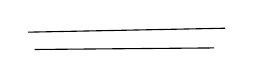
\begin{tikzpicture}\draw (0,.12)--(2.5,.17); \draw (.08,-.1)--(2.36,-.08);\end{tikzpicture}}

4) \quad Ens. de petit cardinal

a) \uline{Cardinal 2}\qquad Ens de cardinal 2 $\longleftrightarrow$ torseur \unsure{sur|sous} $\mathbb{Z}_2$ ou encore, \uline{espace affine \deleted{\unsure{sous}}} $\deleted{\unsure{\mathbb{Z}}}\mathbb{F}_2$ (ou encore, \deleted{\illegible{1}} espace affine de dim 1 sur corps $\mathbb{F}_2$ --- car les espaces vect. de dim 1 sur $\mathbb{F}_2$ sont can. isomorphes \ldots)

\[
\boxed{\operatorname{Aff}(1,\mathbb{F}_2)\simeq
 \operatorname{Aff}(\mathbb{Z}_2)\simeq\unsure{\mathfrak{S}|\mathcal{S}}_{\unsure{2|n}}}
\]
\[
(\unsure{\mathcal{A}|A}_2=\{1\})
\]

b) \uline{Cardinal 3}
\[
\begin{aligned}
\mathfrak{S}_3&\simeq\operatorname{Aff}(1,\mathbb{F}_3)&
 &\simeq\operatorname{Gl}(2,\mathbb{F}_2)&
 &\simeq\operatorname{GP}(1,\mathbb{F}_2)\\
&\hspace{2em}\rotatebox{90}{$\simeq$}&&&&\hspace{3em}\rotatebox{90}{$=$}\\
&\hspace{1em}\mathbb{F}_3^{+}\mathbin{.}\mathbb{F}_3^{*}
 &&&&\operatorname{Gl}(2,\mathbb{F}_2)/\mathbb{F}_2^{*}\\
&\hspace{1em}\rotatebox{90}{$\unsure{\simeq|=}$}
 \quad\rotatebox{90}{$=$}\\
&\hspace{.8em}\mathbb{Z}_3\quad\mathbb{Z}_2
\end{aligned}
\]
\[
\mathcal{A}_3\simeq\deleted{\unsure{\mathbb{Z}}}\mathbb{F}_3^{+}(\simeq\mathbb{Z}_3)
\]
% archive sheet number: 12

\scanpage{14}
c)
\[
\begin{aligned}
\unsure{\mathfrak{S}|\mathcal{S}}_4&\simeq\operatorname{Aff}(2,\mathbb{F}_2)\simeq\operatorname{GP}(1,\mathbb{F}_3)\\
\unsure{\mathfrak{A}|\mathcal{A}}_4&\simeq\operatorname{Aff}(1,\mathbb{F}_4)\qquad ?
\end{aligned}
\]

d)
\[
\begin{aligned}
\mathfrak{S}_5&\simeq\operatorname{GP}(1,\mathbb{F}_5)\\
\mathfrak{A}_5&\simeq\operatorname{GP}(1,\mathbb{F}_4)
\end{aligned}
\]

Quelques groupes classiques sur un corps $k$

\diagram{\(\left.
\begin{tikzcd}[ampersand replacement=\&,column sep=small,row sep=1em]
1\arrow[r] \& k^*\arrow[r] \& \operatorname{Gl}(V)\arrow[r] \&\operatorname{GP}(V)\arrow[r,dash]\&1\\
1\arrow[r] \& k^*\arrow[r,dash] \&\operatorname{Gl}(n,k)\arrow[r] \&\operatorname{GP}(n-1,k)\arrow[r]\&1
\end{tikzcd}
\right\}\;\text{ne \unsure{splitte} pas en général}\)}

% slanted
\margin{\tikz[baseline=(proj.base)]{\node[inner sep=2pt] (proj) {\shortstack{$\unsure{\mathbb{P}|P}(V)\simeq V/k^*$\\$\operatorname{GP}(V)$ opère\\dessus}}; \draw (proj.center) ellipse [x radius=1.22cm,y radius=.94cm];}}

Structure de $k$-vectoriel \inserted{de dim $n$} sur ens $V$ $\longleftrightarrow$ donnée d'\unsure{un|une} \unsure{élémt|élément} de $\operatorname{Isom}_{\text{ens}}(k^n,V)/\operatorname{Gl}(n,k)$

Structure de $k$-espace affine de dim $n$ sur \deleted{\unsure{$E$}} ens $E$
\[
\longleftrightarrow\ \text{donnée d'un élément de}\quad
\operatorname{Isom}_{\text{ens}}(k^n,V)/\operatorname{Aff}(n,k)
\]

[ De façon \unsure{générale|général}, \deleted{si $Z$ est un groupe}, la notion de \deleted{espace affine}\inserted{torseur (à droite, disons) $E$} sous groupe non précisé peut être considéré comme structure sur le seul ens de base $E$, \deleted{\unsure{savoir application} $E\times E\times E\mathbin{\text{---}}E$}\inserted{p.ex. donnée d'un} \deleted{$(x,y,z)\longmapsto\unsure{6x|sx}$} couple $\Gamma\subset\mathfrak{S}_{E}$ ss-grpe, tel que \ldots ] ; valable pour ens. à grpe d'op \uline{fidèle}\ldots ]

Une structure d'\uline{espace affine sous} $k$ est alors la donnée d'un tel $\Gamma$, avec \deleted{\unsure{$\Gamma$ com}} comm, \deleted{et} un hom d'anneaux unit.
\[
 k\longrightarrow\operatorname{End}_{\mathbb{Z}}(\Gamma)\quad\ldots\qquad ]
\]

Structure de $k$-espace projectif de dim $n$ sur $\unsure{P|\mathbb P}$
\[
\overset{\substack{\boxed{\text{déf}}\\\downarrow}}{\longleftrightarrow}
\ \text{donnée de}\quad
\operatorname{Isom}_{\text{ens}} \left(
 \underset{\substack{\rotatebox{90}{$=$}\\(k^n-\unsure{(0)|\{0\}|0}/k^*}}{\mathbb{P}^{n-1}(k)},P\right)
 /\operatorname{GP}(n-1,k)
\]

\figure{
\begin{tikzpicture}[x=\linewidth,y=1ex]
\draw (.29,1.5) -- (.58,1.5) .. controls (.61,1.5) and (.61,-.5) .. (.65,-.5) -- (.98,-.5);
\end{tikzpicture}}
\diagram{\begin{tikzcd}[ampersand replacement=\&,column sep=small,row sep=.6em]
\operatorname{Gl}(n,k)\arrow[r]\&\operatorname{Aff}(n,k)\arrow[r]\&\operatorname{GP}(n,k)\\
\substack{\text{vect. de dim $n$}\\\text{sur $k$}}\arrow[r,maps to,"\substack{\text{oubli}\\\text{origine}}"']
\&\substack{\text{espace affine de}\\\text{dim $n$ sur $k$}}
\arrow[r,maps to,"\substack{\text{espace proj.}\\\text{associé à}\\\text{l'esp. vect. \unsure{enveloppant|enveloppe}}}"']
\&\substack{\text{espace projectif}\\\text{de dim $n$ sur $k$}}
\end{tikzcd}}
% archive sheet number: 13

\scanpage{15}
\uline{Exercice}\qquad Réalisation régulière d'un polygône.

Soit $\deleted{\unsure{V}}E$ plan affine euclidien sur $\unsure{\mathbb{R}|R}$ (avec métrique déf pos. sur l'espace $V$ des translations). Une réalisation rectiligne d'un polygone $(S,A,R)$ est dite \uline{régulière} si tous les \unsure{cotes|cotés|côtés} du polygône ont $=$ longueur\inserted{\tikz[baseline=(angle.base)]{\node[inner sep=1.7pt] (angle) {\shortstack{et tous les angles\\itou}}; \draw (angle.north west) .. controls +(1em,.1em) and +(-.4em,.2em) .. (angle.north east) .. controls +(.4em,-.45em) and +(.2em,0) .. (angle.south east) .. controls +(-.65em,-.4em) and +(0,.3em) .. (angle.south west) -- ([xshift=-.45em]angle.west) .. controls +(.35em,.7em) and +(-.45em,0) .. (angle.north west);}}, régulière \deleted{\unsure{et}} \uline{normalisée} si la dite longueur est 1.

a) Existence, grâce à équation cyclotomique $z^n=1$ dans $\unsure{\mathbb{C}|C}$.

b) Prouver que si $(V\deleted{\unsure{,}}\supset P\deleted{\unsure{,}}\supset\deleted{\unsure{A}}S)$ et $(V'\supset P'\supset S')$ sont deux $n$-polygônes ($n\geq3$) munis d'une \unsure{réal.} rectiligne \uline{rég.} (resp normalisée) il existe une \deleted{\unsure{iso}} similitude (resp \unsure{isom}) \deleted{\uline{unique}} de $V$ sur $V'$, qui transforme $P$ \unsure{et|en} $P'$, $S$ en $S'$; \deleted{\unsure{si $V,P,S$}} plus précisément, pour tt isom (comb) de $(\deleted{\unsure{P}}S,A,R)$ sur $(S',A',R')$, $\exists\,\unsure{\vert|1}$ similitude \inserted{(isom)} de $\deleted{\unsure{E}}V$ sur $V'$ qui l'induise. \deleted{Montrer que}

\deleted{\unsure{Ex|Cor}}\quad\uline{Cor} Notion d'enveloppe affine (ou vectorielle, grâce : centre de gravité \inserted{de l'ens des sommets}) d'un polygône combinatoire.

\deleted{\unsure{Soit|Si}} Orientation du polygône $\longleftrightarrow$ orientation de son enveloppe
% archive sheet number: 14

\scanpage{16}
Polygône régulier (ou réalisation régulière d'un polygône combinatoire) : définitions possibles (\unsure{cotés|côtés} égaux, angles égaux, \inserted{\deleted{\unsure{il suffit|il faut|il y avait}} les deux,} transitivité groupe des symétries ...) Existence, unicité modulo homothétie : tout isom. combinatoire est induit par une unique similitude.

\figure{\begin{tikzpicture}[x=.8cm,y=.8cm]
\draw (0,0) -- (1.14,.66);
\draw (1.18,.70) -- (1.55,1.97);
\end{tikzpicture}}

Notion d'enveloppe affine (ou vectorielle) d'un polygône combinatoire ... \unsure{sens} précisé

\noindent\hfil\rule{.24\linewidth}{.35pt}\hfil\par
Fonctorialité de $X\times_G Y$ \unsure{p.r.} à $(\unsure{G|X},X,Y)$ ...
\par\noindent\hfil\rule{.27\linewidth}{.35pt}\hfil\par

\[
\begin{aligned}
\unsure{P|\overline{P}|T}\times_G E={}^{P}\!\deleted{\unsure{B}}E=F
&\qquad\qquad &P&\quad G\text{-torseur}\\
&&E&\quad G\text{-ensemble}
\end{aligned}
\]

$P\longrightarrow\operatorname{Bij}(E,F)$ compatible aux opérations de $G$ à droite

\uline{NB} Si $\unsure{G}$ opère fidèlement sur $E$, $G$ opère ``sans pts fixes'' sur $\operatorname{Bij}(E,F)$ --- i.e. $\deleted{\unsure{y}}\unsure{x|y}.g=\unsure{x|u}$ $(g\in G,\ x\in B)$ implique $g=1$, ou encore les $G_x$ $(x\in B)$ sont réduits à $\{1\}$, ou encore $B$ est une somme de torseurs ... Dans ce cas\inserted{ et dans ce cas seulement}, $P\mathbin{\text{---}}\operatorname{Bij}(E,F)$ est injectif

\[
P\hookrightarrow\operatorname{Bij}(E,F)
\]

% slanted
\margin{\tikz[baseline=(side.base)]{
\node[inner sep=1pt] (side) {\shortstack[l]{$(G,E)$-structure\\sur ens $F$}};
\draw (side.south west) .. controls +(1em,-.3em) and +(-.35em,.7em) .. ([xshift=-.04em,yshift=-.5em]side.south)
 .. controls +(.3em,.8em) and +(-.8em,-.3em) .. (side.south east);
\node[anchor=north east,inner sep=1pt] at ([xshift=-.2em,yshift=-.25em]side.south) {\deleted{\illegible{1}}};
\draw ([yshift=-.57em]side.south) -- ++(0,-2em) .. controls +(0,-.4em) and +(-.3em,0) .. ++(.55em,-.5em);}}
\noindent$\left[\begin{minipage}{.84\linewidth}
En tous les cas, $F\inserted{={}^{P}\!E}$ est muni de la structure suivante : donnée d'une orbite de $G$ dans $\operatorname{Bij}(E,F)$.
\end{minipage}\right.$

{\footnotesize [On verra que (si $G$ opère $\unsure{\text{fid}^{\mathrm{t}}}$ sur $E$) la donnée d'un \deleted{\unsure{ens|d'un}} \deleted{\unsure{$(G,E)$-st}} $\unsure{F}$ avec $(G,E)$-structure \unsure{équivaut à|équiv. à} celle d'un \unsure{$G$-torseur} \unsure{et applic$^{\mathrm{tn}}$}.]}

\uline{Corollaire} \unsure{de|du} $\unsure{\big[\,\mathbin{\text{---}}|\big[\,\longrightarrow}$ \unsure{toute structure}
% archive sheet number: 15

\scanpage{17}
sur $E$ invariante par $G$ est transportée sur $F$.

(Ex : structures de groupe, d'anneau, de module sur un anneau fixé, d'espace top. etc ...)

Cas de plusieurs ens de base $(E_i)_{i\in I}$ \deleted{\unsure{$E$ muni}} \unsure{muni|munis} d'une structure mixte (p.ex. module $E$ sur anneau $A$, $G$ opère sur $(A,E)$) alors $({\scriptstyle\unsure{1|\prime}}{}^{\unsure{P|\overline P|T}}\!E_i)_{i\in I}$ sont munis de la structure correspondante.

\deleted{\uline{\unsure{NB}}}

\uline{\deleted{\unsure{M}}Applications}\quad \deleted{\unsure{Méth.|Mét.}}\inserted{\tikz[baseline=(n.base)]\node[draw,circle,inner sep=1.2pt] (n) {1};} Yoga : structures isomorphes : Une \inserted{\unsure{str}} donnée $E$ $\longleftrightarrow$ torseurs sous $G=\operatorname{Aut}(E)$

\diagram{\begin{tikzcd}[ampersand replacement=\&,row sep=1.1em,column sep=1.15em]
F \arrow[r,maps to] \& \operatorname{Isom}_{\unsure{e|C|G|\mathcal C}}(E,F)=\unsure{\overline P|P}\\
{}^{P}\!E=P\times_G E \& P \arrow[l,maps to]
\end{tikzcd}}

\diagram{\begin{tikzcd}[ampersand replacement=\&,column sep=1.15em,row sep=.4em]
F \& \unsure{\longmapsto|\mathrel{\vdash\!\!-}} \& P^{\unsure{\cdots}}\arrow[d,dash]\arrow[r,maps to] \& P\times_G E\arrow[r,"{\overset{?}{\sim}}"] \& F\\
\& \& \operatorname{Isom}_{C}(E,F) \& \&
\end{tikzcd}}

\[
\begin{aligned}
P\times E&\longrightarrow F\\
\operatorname{Isom}(E,F)\times E&\mathbin{\text{---}} F
  & (u,x)&\ \unsure{\mathrel{\vdash\!\!-\!\dashv}|\longmapsto}\ u(x)\\
&& (ug)(\unsure{x|u})&=u(gx)\qquad\text{ok}
\end{aligned}
\]

\diagram{\begin{tikzcd}[ampersand replacement=\&,row sep=.65em,column sep=.85em]
P\arrow[r] \& F=P\times_G E\arrow[r,maps to] \& \operatorname{Isom}_{C}(E,F) \& P\arrow[l,"\sim"']\\
\& \& i_u:x\longmapsto u*x \& \unsure{u|x}\arrow[l,maps to]
\end{tikzcd}}

\[
\deleted{\unsure{(ug}}\,i_{ug}=i_u.g\qquad\text{i.e.}\quad ug*x=u*gx\quad\text{ok}
\]
% archive sheet number: 16

